\documentclass{article}
\usepackage{amsmath}
\usepackage{amssymb}
\usepackage{tikz}
\usepackage{cancel}
\usepackage[hidelinks]{hyperref}

\begin{document}
\begin{titlepage}
    \vspace{20mm}
    \begin{center}
        \Huge \textbf{Appunti di Elaborazione dei Segnali} \\
        \medskip
        \LARGE By \textit{@Thisisfava}\\
        \medskip
        \large 2024/2025
    \end{center}
\end{titlepage}
\newpage
\addcontentsline{toc}{section}{}
\tableofcontents
\newpage
\section{Intelligenza}
Dare una definizione generale e universale di intelligenza è davvero difficile, 
dal momento che l'intelligenza può manifestarsi in diversi modi e atteggiamenti. 
è stata data, tuttavia una \textbf{definizione operativa} che permette di descrivere diverse intelligenze rispetto a \textbf{come fare} e \textbf{cosa fare}.
\subsection{Definizione Operativa}
La definizione operativa di cui parlavo prima è riassumibile nella seguente tabella
\begin{table}[h]
    \centering
    \begin{tabular}{|c|p{5cm}|p{5cm}|}
        \hline
         & \textbf{Umanamente} & \textbf{Razionalmente} \\ \hline
        \textbf{Pensare} & Codificare il funzionamento della mente in un programma & Un programma che usa deduzioni logiche per risolvere il problema \\ \hline
        \textbf{Agire} & Un programma che ha comportamento umano & Un programma che prende "buone" decisioni \\ \hline
    \end{tabular}
\end{table}

\paragraph{Pensare Umanamente.} Consiste nel ottenere un programma che pensa come il nostro cervello; 
è impossibile dal momento che ancora oggi non lo conosciamo del tutto.
\paragraph{Pensare Razionalmente.} Consiste nel formalizzare tutta la conoscenza tramite assiomi/regole logiche per poter dedurre/inferire ragionamenti
\paragraph{Agire Umanamente.} Consiste nell'emulare il comportamento umano (sbagliando, commettendo imprecisioni, ecc...). I captcha sfruttano questa capacità per distinguere i bot dagli umani.
\paragraph{Agire Razionalmente.} Consiste nella capacità da parte dell'agente di prendere delle decisioni che lo portano al raggiungimento dei suoi obiettivi. \\\textbf{Nota Bene: }Questa è la definizione che utilizzeremo nel corso. 

\subsection{Problema dell'agire umanamente}
Per quanto possa essere facile da realizzare e utile un agente che agisce umanamente (perchè quest'intelligenza è profondamente legata al task per il quale sono costruiti), esiste un problema che li affligge (soprattutto nei casi più complessi): 
l'impossibilità di determinare il percorso di ragionamento che ha portato l'agente a prendere questa o quella decisione. 
Il problema è così critico che l'intera industria dell'autonomous driving è stata rallentata.  


\subsection{Test di Turing}
Spesso, tuttavia, la tabella sopra proposta risulta essere poco pratica e molto astratta. 
Alan Turing propose, invece, un esperimento che permettesse di determinare se l'agente è intelligente o meno a partire dall'essere intelligente (si spera ) per definizione: l'essere umano. 
Una formulazione del Test di Turing è la seguente:\\
Dati A e B agenti intelligenti (tipicamente un uomo e una donna), e C l'agente di cui testare l'intelligenza:
\begin{itemize}
    \item C deve indovinare il sesso di A e B
    \item B collabora con C
    \item A inganna C
\end{itemize}
Se swappando A con B si ottengono le stesse percentuali di successo, l'agente pensa umanamente.
Questo perchè, per superare il test l'agente dovrebbe possedere le seguenti capacità: 
\begin{itemize}
    \item \textbf{interpretazione del linguaggio naturale} per comunicare con l'esaminatore 
    nel suo linguaggio umano    
    \item \textbf{rappresentazione della conoscenza} per memorizzare quello che sa o sente
    \item \textbf{ragionamento automatico} per utilizzare la conoscenza memorizzata in modo 
    da rispondere alle domande e trarre nuove conclusioni
    \item \textbf{apprendimento} per adattarsi a nuove circostanze, individuare ed estrapolare pattern
\end{itemize}
\newpage
\subsection{Operazioni nel campo dei complessi}
\subsubsection{Somme tra numeri complessi}
\paragraph{Forma algebrica.} Dati $z_1 = x_1 + jy_1$ e $z_2 = x_2 + jy_2$ la somma sarà:
\begin{equation}
    z_1 + z_2 = (x_1 + x_2) + j(y_1 + y_2)
\end{equation}
\paragraph{Forma Esponenziale.} La somma è banale

\subsubsection{Scalatura}
\paragraph{Forma algebrica.} Dati $z = x + jy$ e $a \in \mathbb{R}$ la scalatura sarà:
\begin{equation}
    az = ax + jay
\end{equation}
\paragraph{Forma Esponenziale.} Dati $z = \rho e^{j\theta}$ e $a \in \mathbb{R}$ la scalatura sarà:
\begin{equation}
    az = a\rho e^{j\theta}
\end{equation}


\subsubsection{Prodotto tra complessi}
\paragraph{Forma algebrica.} Dati $z_1 = x_1 + jy_1$ e $z_2 = x_2 + jy_2$ il prodotto sarà:
\begin{equation}
    z_1 \cdot z_2 = (x_1x_2 + y_1y_2) + j(x_1y_2 + x_2y_1)
\end{equation}
\paragraph{Forma Esponenziale.} Dati $z_1 = \rho_1 e^{j\theta_1}$ e $z_2 = \rho_2 e^{j\theta_2}$ il prodotto sarà:
\begin{equation}
    z_1 \cdot z_2 = \rho_1 \rho_2 e^{j(\theta_1 + \theta_2)}
\end{equation}

\subsubsection{Inverso di un complesso}
\paragraph{Forma algebrica.} Dato $z = x + jy$ l'inverso sarà:
\begin{equation}
    \frac{1}{z} = \frac{\overline{z}}{\rho^2} = \frac{x - jy}{x^2 + y^2}
\end{equation}
Spiegazione della formula: un certo $w = z^{-1}$ con $z \in \mathbb{C}$ se il loro prodotto genera un numero con parte reale unitaria e parte immaginaria nulla.
Sappiamo che $z\cdot \overline{z} = x^2 + y^2 = \left\lvert z\right\rvert = \rho^2$. Quindi basta dividere il coniugato di z con il modulo quadro($\rho^2$) e si ha l'inverso.
\paragraph{Forma Esponenziale.} Dati $z = \rho e^{j\theta}$ il prodotto sarà:
\begin{equation}
    \frac{1}{z} = \frac{1}{\rho} e^{-j\theta}
\end{equation}

\subsubsection{Divisione tra numeri complessi}
Dati $z_1 \in \mathbb{C}$ e $z_2 \in \mathbb{C}$ possiamo riscrivere la divisione tra i 2 numeri come prodotto tra il primo e l'inverso del secondo, e ciò vale per entrambe le forme:
\begin{equation}
    \frac{z_1}{z_2} = z_1 \cdot \frac{1}{z_2}
\end{equation}


\subsubsection{Elevamento a potenza}
\paragraph{Forma algebrica.} L'elevamento ha potenza della forma algebrica non è particolarmente interessante.
\paragraph{Forma Esponenziale.} Dati $z = \rho e^{j\theta}$ e $n \in \mathbb{Z}$ l'elevamento a potenza sarà $z ^ n = \underbrace{z\cdot z\cdot \ldots \cdot z}_{\mbox{n volte}}$ ossia:
\begin{equation}
    z^n = \rho^ne^{jn\theta}
\end{equation}


\subsubsection{Estrazione di una radice n-esima}
Dato un $z \in \mathbb{C}$ e $y \in \mathbb{C}$, $y$ è radice n-esima di z se e solo se $y^n = z$. 
La grande differenza con in numeri reali è che, nel campo complesso, esistono esattamente $n$ y distinte di radici che soddisfano l'equazione $y^n - z = 0$ per il teorema fondamentale dell'algebra.  
\paragraph{Forma algebrica.} La radice n-esima della forma algebrica non è particolarmente interessante.
\paragraph{Forma Esponenziale.} Dati $z = \rho e^{j\theta}$ e $n \in \mathbb{N}$ la radice n-esima sarà:
\begin{equation}
    \sqrt[\leftroot{-2}\uproot{2}n]{z} = \sqrt[\leftroot{-2}\uproot{2}n]{\rho}e^{j\left(\frac{\theta + 2\pi i}{n}\right)} \tag*{\small Con i = 0,1,\dots, n-1 \normalsize}
\end{equation}

\subsubsection{Funzione complessa di variabile reale}
Definita come
\begin{equation*}
    f : \mathbb{R} \longrightarrow \mathbb{C}
\end{equation*}
Oppure come $z = f(x)$ con $z \in \mathbb{C}$ e $x \in \mathbb{R}$, è una funzione che mappa ad ogni reale un immaginario.
\paragraph{Rappresentazione.}Graficamente una funzione complessa di variabile reale può essere rappresentata in un grafico a 3 dimensioni con un asse per la x (variabile indipendente) e gli altri 2 assi sono $\mathbb{I}m[z]$ e $\mathbb{R}e[z]$.
Dal momento che sono difficili da rappresentare, si ricorre ad una semplificazione: il grafico tridimensionale si sdoppia in un grafico che mappa ad ogni $x$ la parte Reale di z ed un altro grafico che mappa ad ogni x la parte Immaginaria di z.
Se si lavora in coordinate polari, è possibile invece rappresentare il grafico che mappa ad ogni x il modulo del complesso corrispondente e un altro grafico che mappa ad ogni x la fase del complesso corrispondente. La particolarità di questi ultimi 2 grafici è che il primo grafico è sempre rappresentato sopra l'asse x (il modulo non può mai essere negativo) e il secondo grafico è sempre rappresentato tra $-\pi$ e $\pi$ dal momento che poi la fase si ripete.
\newpage
\subsection{Tipi di Agenti}
\subsubsection{Agente Reflex}
\lezione{Lezione 3}{7/10/2024}
L'agente reattivo è sicuramento quello più semplice (ma anche usato): è basato sulla statica mappatura 
di percezione-azione. La particolarità di questo agente è l'assenza di stato: la mappatura non cambierà mai perchè 
non viene tenuta in considerazione lo storico delle percezioni (è come se fosse un circuito combinatorio, una funzione ben definita).

\subsubsection{Agente Reflex con Modello}
Più adatto in ambienti parzialmente osservabili, l'Agente Reflex con Modello tiene traccia della parte dell'ambiente che non può osservare nell'istante corrente.
Per poter far ciò, l'agente deve poter conoscere:
\begin{itemize}
    \item \textbf{Le leggi che descrivono l'ambiente}: (o quelle sufficienti) per poter determinare come può evolvere l'ambiente a prescindere dalle azioni
    \item \textbf{Gli effetti delle azioni}: per poter determinare l'effetto delle azioni dell'agente sull'ambiente 
\end{itemize}
Questi 2 tipi di conoscenza vengono detti \textbf{Modelli del Mondo}

\subsubsection{Agente basato su Goal}
Un altro tipo di Agente è quello basato su Goal, ossia, quello che conosce l'obiettivo da raggiungere e deve poter calcolare, per ogni azione
quanto l'agente si avvicina a tale obiettivo. Questa operazione è semplice se il calcolo si può fare in pochi passi, ma se si deve valutare lo storico
delle azioni, in questo caso non lo è più. Esiste un'intera branca dell'IA che si occupa della Ricerca e Pianificazione.\\ 

Il concetto di obiettivo, tuttavia, è limitante: in base ad un obiettivo si possono scartare gli stati che ci allontanano e gli stati che ci fanno avvicinare all'obiettivo, ma ancora è difficile \textbf{quantificare} la distanza dall'obiettivo.
Esistono diversi parametri che possiamo utilizzare per quantificare la bontà di un'azione:
\begin{itemize}
    \item \textbf{Valore Atteso}: Un primo che viene usato per quantificare la bontà di un'opzione tra le tante è il valore atteso (il prodotto tra la vincita e la sua probabilità, prendendo come esempio quello della lotteria)
    \item \textbf{Propensione/Avversione al rischio}: un altro parametro riguarda quanto è propenso al rischio l'agente; in base a quello si può prediligere la minima vincita con alta probabilità o massima vincita con bassa probabilità
    \item \textbf{Utilità}: questo parametro permette di quantificare quanto è utile un premio rispetto ad un altro (es: 100\$ per un povero sono molto utili. Per un ricco, invece, sono poco utili).
\end{itemize}


\subsubsection{Agente basato su Utilità}
Un agente basato su Utilità è un agente con modello le cui decisioni vengono prese non per raggiungere un obiettivo, ma per massimizzare il grado di "contentezza" dell'agente stesso.
Per apprezzare meglio il concetto di Utilità e come questo abbia avuto importanti ripercussioni in ambito IA è necessario introdurre una serie di formalismi.

\subsection{Relazione di Preferenza}
\subsubsection{Definizioni}
\begin{itemize}
    \item $\displaystyle S = \{s_1, s_2, \dots\}$ insieme degli stati possibili
    \item $\displaystyle s_i \succeq s_j $ è detta \textbf{preferenza debole} di $s_i$ a $s_j$
    \item $\displaystyle s_i \succ s_j$ è detta \textbf{preferenza (stretta)} di $s_i$ a $s_j$
    \item $\displaystyle s_i \thicksim  s_j$ è detta \textbf{indifferenza} di $s_i$ a $s_j$
\end{itemize}

Grazie alla probabilità e alle definizioni precedenti è possibile definire il concetto di \textbf{Lotteria} $l$ (che può essere vista anche come una funzione di massa):
\begin{equation}
    l = [p_1:s_1, p_2:s_2, \dots]
\end{equation}
dove $s_i$ è il possibile esito della lotteria, $p_i:s_i$ è la probabilità che si verifichi $s_i$.
Inoltre è necessario che $\sum_{i} p_i = 1$

\subsubsection{Proprietà}
Affinchè una relazione sia di preferenza deve rispettare le seguenti proprietà
\begin{itemize}
    \item \textbf{Completezza}: è necessario che ogni preferenza sia comparabile
        \begin{equation} \label{prop: C}
            s_1 \succ s_2 \vee s_1 \succeq s_2 \vee s_1 \thicksim s_2 \quad \forall s_1, s_2 
        \end{equation}
    \item \textbf{Transitività}: Dati $s_1 \succ s_2 \mbox{ e } s_2 \succ s_3$ allora:
        \begin{equation} \label{prop: T}
            s_1 \succ s_3 
        \end{equation}
    \item \textbf{Sostituibilità}: Dati 2 stati $s_a$ e $s_b$ indifferenti, le lotterie, che contengono sia il primo stato che il secondo stato
    con la stessa probabilità $q$, devono essere altrettanto indifferenti
    \begin{equation} \label{prop: S}
        [q:s_a,p_1:s_1, \dots] \thicksim [q:s_b, p_1:s_1, \dots] \quad \mbox{se } s_a \thicksim s_b
    \end{equation}
    Inoltre è necessario che $q + \sum_i p_i = 1$
    \item  \textbf{Decomponibilità (Not Fun In Gambling)}: giocare alle varie lotterie in una qualsiasi sequenza non deve influenzare le probabilità di vincita.
    In parole povere, le varie sottolotterie di una lotteria devono essere indipendenti tra loro. Formalizzando:\\
    Detta $p_i^e$ la probabilità con cui la lotteria $e$ seleziona lo stato $s_i$, allora date 2 lotterie $l_1,l_2$ se $l_1 \thicksim l_2$ allora
    \begin{equation} \label{prop: D}
        p_i^{l_1} = p_i^{l_2}
    \end{equation} 

    \item \textbf{Monotonicità}: Dati stati preferibili e delle probabilità, la lotteria preferibile è quella che assegna la probabilità maggiore allo stato più preferibile, ossia:\\
    Se $ s_1 \succ s_2 $ e $p > q$ allora:
    \begin{equation} \label{prop: M}
        [p:s_1,(1-p):s_2] \succ [q:s_1,(1-q):s_2]
    \end{equation}

    \item \textbf{Continuità}: Dati 3 stati, uno più preferibile dell'altro, esisterà sempre un valore tra 0 e 1 che renda la lotteria, tra il più preferibile e il meno preferibile, indifferente allo stato "intermedio", ossia:\\
    Dati $s_1 \succ s_2 \succ s_3$, $\exists p \in [0,1]$ tale che:
    \begin{equation} \label{prop: CC}
        s_2 \thicksim [p: s_1, (1-p): s_3]
    \end{equation}
\end{itemize}


\subsection{Teorema di Neumann-Morgenstein}
Data una relazione di preferenza che rispetta le proprietà \eqref{prop: C},\eqref{prop: T},\eqref{prop: S},\eqref{prop: D},\eqref{prop: M},\eqref{prop: CC} 
allora $\exists u: \mathcal{L} \longrightarrow [0,1]$ (dove $\mathcal{L}$ è l'insieme delle possibili lotterie) tale che:
\begin{equation}
        s_1 \succ s_2 \Longleftrightarrow u(s_1) > u(s_2)
\end{equation}
\begin{equation}
    u([p_1:s_1, \dots]) = \displaystyle \sum_i p_i u(s_i)
\end{equation}
La $u$ viene detta \textit{funzione di utilità} mentre $u(s_i)$ è detta \textit{utilità dello stato i}.
In parole povere, il teorema afferma che, data una relazione di preferenza che rispetta quelle proprietà, è possibile definire
una funzione che associa ad ogni stato un'utilità, dunque se uno stato è preferibile ad un altro, la sua utilità sarà maggiore; inoltre l'utilità di una lotteria è definibile come il valore atteso della funzione utilità. Dunque, per raggiungere lo stato di massima felicità, l'agente deve massimizzare una funzione (che è appunto $u$).
Dunque, grazie a questo importante teorema, siamo riusciti a ricondurre una forma di ragionamento nella massimizzazione di una funzione (che è un problema facilmente attaccabile)
\newpage
\section{Problemi di Search}
L'insieme dei problemi di Search è un insieme di problemi legati all'inferenza (piuttosto che al Machine Learning). 
Tali problemi vengono formulati e risolti da un agente per trovare il percorso che li porterà ad uno stato obiettivo;
per fare ciò, considereremo un ambiente che è:
\begin{itemize}
    \item \textbf{Statico} dal momento che assumiamo che durante la ricerca il mondo non cambi (altrimenti la ricerca sarà inutile)
    \item \textbf{A Singolo Agente} per semplificare la situazione
    \item \textbf{Completamente Osservabile} per poter conoscere lo stato iniziale dell'agente
    \item \textbf{Discreto} in modo da poter descrivere i passi risolutivi in maniera discreta
    \item \textbf{Deterministico} perchè ad ogni azione devo essere sicuro del suo effetto per la computazione dello stato successivo
\end{itemize}
\subsection{Formulazione del Problema}
Per la descrizione dei problemi di Search useremo queste convenzioni:
\begin{itemize}
    \item $S = \{ s_1, s_2, \dots\}$ è detto \textit{Insieme degli stati} (deve essere finito)
    \item $s_i \in S$ è detto \textit{stato iniziale}
    \item $s_G \in S$ è detto \textit{stato di Goal} (può essere più di uno)
    \item $A(s_i) = \{ a,b,c,\dots\}$è \textit{l'insieme delle azioni possibili allo stato i}
    \item $f(s_i,a)$ con $s_i \in S$ e $a \in A(s_i)$ è detto \textit{modello di Transizione} o \textit{Funzione Successore}; corrisponde allo lo stato successivo
    \item $c(s_i,a,f(s_i,a))$ è detto \textit{costo Additivo}. Una cosa da tenere a mente per il costo additivo
    è che i vari costi devono poter essere tutti sommabili (non possono essere grandezze diverse)
\end{itemize}

Un'altra formulazione interessante del problema usa il \textit{Grafo degli Stati}, dove gli archi sono le azioni e i nodi sono gli
stati.

\subsection{Classificazione dei problemi}
In base a cosa cercare, i problemi di Search possono essere di 3 tipi:
\begin{itemize}
    \item \textbf{Fattibilità} \label{def:fattibilità} \\ 
    I problemi di Fattibilità hanno come obiettivo di rispondere la domanda: \textit{Esiste un percorso che mi porta da $s_i$ ad un $s_G$?}.
    In questi problemi bisogna quindi esplorare un qualunque percorso che mi porti all'uscita del labirinto, senza sapere necessariamente la sequenza di azioni o quella più efficiente/interessante.
    \item \textbf{Approssimazione}\\
    I problemi di Approssimazione, invece, ricercano una soluzione che soddisfi alcune garanzie (es: "il percorso trovato dev'essere al massimo il 30\% peggiore dell'ottimo").
    Chiaramente questi tipi di algoritmi sono difficili da progettare dal momento che dimostrare tali garanzie è davvero arduo.
    \item \textbf{Ottimizzazione}\\
    Sono problemi che richiedono il percorso più bello/efficiente/interessante rispetto a tutti gli altri (e di dimostrarlo) che mi porti allo stato obiettivo.
\end{itemize}
In generale dobbiamo dire che, negli ultimi 2 casi, il risultato del problema di Search è un \href{https://it.wikipedia.org/wiki/Albero_(informatica)}{albero} la cui radice è lo stato iniziale e in cui un ramo porta allo stato obiettivo.

\subsection{Approccio Esaustivo/Esplicito}
Un primo approccio che potremmo formulare, per risolvere tali problemi, è quello di
precalcolare tutti i possibili percorsi e selezionare quello più efficiente. Chiaramente questo approccio è INUTILIZZABILE
in problemi di dimensione reale (ma nemmeno troppo grandi): tutti i possibili passi per la risoluzione del Cubo di Rubik, per esempio, sono
circa $4,33 * 10^{43}$ permutazioni, cosa che non è possibile contenere tutta in memoria.

\subsection{Approccio Implicito}
In questo caso, invece, piuttosto che enumerare tutti i possibili percorsi, si esplorano solo quelli più "interessanti" a partire dallo stato iniziale. Dunque,
piuttosto che tenere in memoria tutti i possibili percorsi, tengo solo quelli che effettivamente ho esplorato ed eventualmente scarto quelli non ottimi.

\subsection{Caratteristiche di un Algoritmo}
D'ora in poi, gli algoritmi di Search che mostreremo nel corso verranno valutati in base ai seguenti parametri:
\begin{itemize}
    \item \textbf{Correttezza}: questa proprietà afferma che, se l'algoritmo restituisce un risultato, questo dev'essere conforme alle specifiche 
    (cioè, se si richiede, per esempio, di trovare il percorso migliore, il risultato dell'algoritmo DEVE RESTITUIRE IL PERCORSO MIGLIORE)
    \item \textbf{Completezza}: se esiste una soluzione al problema, l'algoritmo la troverà sempre. In altri termini, l'algoritmo deve sempre terminare con una risposta in un tempo finito. 
    Nel caso in cui i passi del problema sono infiniti (ovviamente contabili), la completezza viene detta \textbf{Sistematicità} e va dimostrata.
    \item \textbf{Complessità Spaziale}: l'uso (nel caso peggiore) della risorsa spaziale (memoria disponibile) per la risoluzione del problema in funzione della dimensione dell'input
    \item \textbf{Complessità Temporale}: l'uso (nel caso peggiore) della risorsa temporale (passi da eseguire) per la risoluzione del problema in funzione della dimensione dell'input
\end{itemize}


\subsection{Problema di Riferimento}
Per presentare i seguenti algoritmi, ci riferiremo sempre a questo grafo, in cui gli archi sono bidirezionali 
(ossia, per ogni $X,Y$ stati del problema $c(X,a,Y) = c(Y,b,X)$ con $a$ l'arco di transizione da $X$ a $Y$ e $b$ l'arco di transizione da $Y$ ad $X$) \\
\begin{center}
    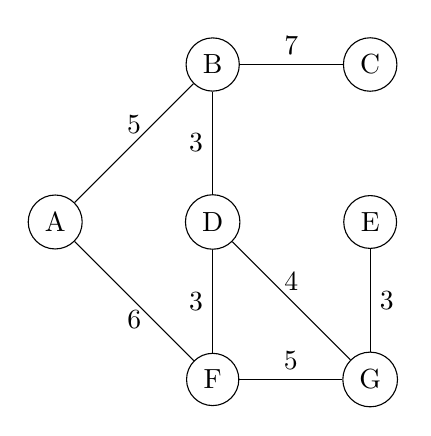
\begin{tikzpicture}
        % Nodi
        \node[circle, draw] (A) at (0,0) {A};
        \node[circle, draw] (B) at (2,2) {B};
        \node[circle, draw] (D) at (2,0) {D};
        \node[circle, draw] (F) at (2,-2) {F};
        \node[circle, draw] (C) at (4,2) {C};
        \node[circle, draw] (G) at (4,-2) {G};
        \node[circle, draw] (E) at (4,0) {E};
    
        % Archi
        \draw[-] (A) -- (B) node[midway, above] {5}; % Arco da A a B
        \draw[-] (A) -- (F) node[midway, below] {6}; % Arco da B a D
        \draw[-] (B) -- (D) node[midway, left] {3}; % Arco da D a C
        \draw[-] (D) -- (F) node[midway, left] {3}; % Arco da C a A
        \draw[-] (B) -- (C) node[midway, above] {7}; % Arco da C a A
        \draw[-] (D) -- (G) node[midway, above] {4}; % Arco da C a A
        \draw[-] (F) -- (G) node[midway, above] {5}; % Arco da C a A
        \draw[-] (G) -- (E) node[midway, right] {3}; % Arco da C a A
    
    \end{tikzpicture}
\end{center}

I vari algoritmi che presenteremo differiscono per come rispondono alla domanda: "\textit{Dato che ho ispezionato il nodo, proseguo o vado indietro?}"


\subsection{Ricerca Non Informata}
\subsubsection{Depth-First-Search}
Un algoritmo classico di ricerca su grafo è la ricerca in profondità. In questa versione, la DFS è dotata di \textit{Backtracking}. Possiamo 
dire in generale che l'approccio di questo algoritmo è aggressiva, poichè ricerca subito in profondità la soluzione (potrebbe metterci molto o potrebbe metterci poco), ossia non c'è garanzia.
Inoltre possiamo osservare che gli alberi generati dalla DFS sono stretti e lunghi.\\
\smallskip
\textbf{Funzionamento:}
\begin{enumerate}
    \item Si parte dal nodo iniziale A (che sarà poi radice dell'albero finale)
    \item Se il nodo da esplorare ha dei figli, si aggiungono all'albero i vari figli; in caso ve ne sia più di uno,
    un \textit{Tie-Breaker} spesso usato è basato sull'ordine lessicografico (quindi, per esempio, se esploriamo A, il primo figlio da esplorare sarà B)
    \item Si torna indietro se: il nodo è foglia, oppure se il nodo è già stato visitato
\end{enumerate}

\textbf{Analisi}:
\begin{itemize}
    \item \textbf{Correttezza}: La dfs restituisce sempre un albero (grazie all'uso del Backtracking e all'eliminazione dei loop)
    \item \textbf{Completezza}: La dfs restituisce sempre un albero in cui un ramo contiene lo stato obiettivo (se esiste il percorso)
    \item \textbf{Complessità Temporale}: Dato b il \textit{Branching Factor} e d la \textit{profondità massima}, la complessità di tale algoritmo è esponenziale, ossia $O(b^d)$
    \item \textbf{Complessità Spaziale}: La memoria usata è quella necessaria per generare l'albero; in questo caso la complessità è $O(d)$ ossia la profondità massima del percorso dallo start al goal.

\end{itemize}

\subsubsection{Breath-First-Search}
Un altro algoritmo classico di ricerca su grafo è la ricerca in ampiezza. Anche la BFS è dotata di \textit{Backtracking}. Possiamo 
dire in generale che l'approccio di questo algoritmo è conservativa, poichè ricerca sempre allo stesso livello, garantendo di visitare tutti i nodi.
Possiamo inoltre dire che gli alberi generati dalla BFS sono larghi e corti.\\
\smallskip
\textbf{Funzionamento:}
\begin{enumerate}
    \item Si parte dal nodo iniziale A (che sarà poi radice dell'albero finale)
    \item Se il nodo padre ha dei figli da esplorare, vengono tutti aggiunti all'albero; Si prosegue poi ai figli del primo nodo figlio e così via.
    Il \textit{Tie-Breaker} che possiamo usare è ancora quello basato sull'ordine lessicografico.
    \item Si torna indietro se: il nodo è foglia, oppure se il nodo è già stato visitato
\end{enumerate}

\textbf{Analisi}:
\begin{itemize}
    \item \textbf{Correttezza}: Per lo stesso motivo della DFS
    \item \textbf{Completezza}: Per lo stesso motivo della DFS
    \item \textbf{Complessità Temporale}: Dato b il \textit{Branching Factor} e q la \textit{profondità minima}, la complessità di tale algoritmo è esponenziale, ossia $O(b^q)$ (quindi sempre minore, nel caso peggiore, della DFS)
    \item \textbf{Complessità Spaziale}: In questo caso, dato che non viene allocata altra memoria se non il grafo stesso, la complessità spaziale sarà $O(n)$ con n il numero di nodi. 
\end{itemize}
\subsubsection{DFS/BFS Ottimizzati}
Gli ultimi 2 algoritmi possono essere ottimizzati introducendo nuove strutture dati, usate per evitare di rivisitare 
i nodi e quindi per generare alberi più piccoli:

\paragraph{EQL (Enqueued List).}
La EQL, anche detta \textit{lista di accodamento}, è una lista che tiene traccia di tutti i nodi già visitati; è detta
di accodamento perchè ad ogni nuova visita, il nodo visitato viene aggiunto alla fine; quando si deve vistare un nodo
si verifica che questo non sia già nella lista; se lo è, tutto il sottoalbero relativo non verrà esplorato. Questa 
operazione è detta \textbf{Potatura} o \textbf{Pruning}

\paragraph{Frontiera.}
Definiamo frontiera l'insieme dei nodi foglia non ancora espansi dell'albero; è detta così dal momento che, per la
\textbf{Separation Property}, separa la parte dell'albero esplorata da quella ancora non esplorata.\\
Implementazioni della Frontiera:
\begin{itemize}
    \item \textbf{Caso BFS}: la frontiera viene implementata come \textbf{Queue} (una coda FIFO)
    \item \textbf{Caso DFS}: la frontiera viene implementata come \textbf{Stack} (una coda LIFO)
\end{itemize}

\textbf{Analisi}:
\begin{itemize}
    \item \textbf{Correttezza}: L'uso delle EQL pota solo i sottoalberi già esplorati, per cui la correttezza non viene compromessa
    \item \textbf{Completezza}: L'algoritmo è ancora completo per il motivo precedente
    \item \textbf{Complessità Temporale/Spaziale}: anche se abbiamo introdotto queste strutture dati per ottimizzare le operazioni,
          in realtà la complessità nel caso peggiore non cambia. Grazie a queste ottimizzazioni, tuttavia, è possibile usare in un tempo ragionevole
          i 2 algoritmi
\end{itemize}

\newpage
\subsection{Proprietà dei Segnali}
\subsubsection{Durata}
La durata di un segnale è, considerando un segnale nel tempo, la differenza tra il primo istante in cui il segnale non è nullo e l'ultimo istante.

\subsubsection{Area}
Si dice \textit{Area di un Segnale} $s(t)$ l'area sottesa dallo stesso segnale, ossia:
\begin{equation}
    \int_{-\infty}^{+\infty} s(t)dt
\end{equation}

\subsubsection{Valor Medio (o Media Temporale)}
Il valor medio di un segnale $s(t)$ non è altro che quel valore $\tilde{s}$ tale che una funzione costante $s'(t) = \tilde{s}$ ha la stessa area di $s(t)$, ossia:
\begin{equation}
    \tilde{s} = \lim_{T \rightarrow +\infty} \frac{1}{2T} \int_{-T}^{+T}s(t)dt
\end{equation}

\subsubsection{Energia}
Sebbene non stiamo parlando propriamente di lavoro e concetti fisici relativi, dobbiamo dire che un segnale è sempre associato ad una certa energia che il segnale stesso trasporta.
Dunque \textit{l'energia di un segnale $(s(t))$} è:
\begin{equation}
    E_s = \int_{-\infty}^{+\infty} |s(t)|^2 dt
\end{equation}

\subsubsection{Potenza Istantanea}
Per il discorso precedente, possiamo anche definire la Potenza Istantanea di un segnale (cioè la potenza in un istante del Segnale) come
\begin{equation}
    P[s(t)] = \begin{cases}
        s(t_0)\overline{s(t_0)} & \mbox{ se } s(t_0) \in \mathbb{C} \\
        s(t_0)^2 & \mbox{ se } s(t_0) \in \mathbb{R}
    \end{cases}
\end{equation}

\subsubsection{Potenza Media}
La potenza media possiamo, invece, vederla come il valore medio dell'energia, ossia:
\begin{equation}
    P_s = \lim_{T \rightarrow +\infty} \frac{1}{2T} \int_{-T}^{+T}|s(t)|^2 dt
\end{equation}

\subsubsection{Segnale Energia e Potenza} \label{def: sep}
Innanzitutto possiamo notare come sia Potenza Media che Energia siano non negativi per costruzione;
inoltre tra Potenza Media e Energia di un segnale è possibile vedere una correlazione: laddove l'energia del segnale è finita, allora la potenza è necessariamente nulla;
laddove invece la potenza media è maggiore di 0, l'energia è infinita.

In base a questo concetto è possibile definire:
\begin{itemize}
    \item \textbf{Segnale Energia} un segnale $s(t)$ se e solo se $0 < E_s < \infty$ e allora $P_s = 0$
    \item \textbf{Segnale Potenza} un segnale $s(t)$ se e solo se $0 < P_s < \infty$ e allora $E_s \rightarrow +\infty$
\end{itemize}

\newpage

\section{Segnali Discreti}
A differenza dei segnali continui, i segnali discreti sono funzioni con Dominio discreto, solitamente rappresentate nella seguente maniera:
\begin{equation*}
    y = f(n), \mbox{  } n \in Z
\end{equation*}
Enunciamo ora tutte le proprietà, in maniera speculare, che abbiamo già descritto per i segnali continui:
\subsection{Operazione sui Segnali Discreti}
\subsubsection{Traslazione}
Dato un segnale $y = f(n)$ definiamo $y' = f(n - n_0)$ traslazione in avanti di $n_0$; definiamo invece $y'' = f(n + n_0)$ traslazione indietro di $n_0$.
\subsubsection{Decimazione/UpSampling}
Dato $y=f(n)$ il segnale con $n \in \mathbb{Z}$, il segnale decimato è:
\begin{equation}
    y = f(an) \mbox{ con } a \in Z \mbox{ e } |a| \geq 1 
\end{equation}
Questa operazione è detta \textit{decimazione} dal momento che è come se prelevassi selettivamente i valori ogni $a$ campioni del segnale di partenza

\subsubsection{Interpolazione/DownSampling}
Dato $y=f(n)$ il segnale con $n \in \mathbb{Z}$, il segnale interpolato è:
\begin{equation}
    y = f\left(\frac{n}{a}\right) \mbox{ con } a \in Z \mbox{ e } |a| \geq 1 
\end{equation}
In parole povere, questa operazione non fa altro che distanziare ogni campione di $a$ intervalli.

\newpage

\subsection{Segnali Notevoli}
\subsubsection{Rettangolo Discreto}
Viene definito come:
\begin{equation}
    rect\left(\frac{n}{D}\right) = \begin{cases}
        1 & \mbox{ se } |\frac{n}{D}| \leq \frac{1}{2}\\
        0 & \mbox{ altrimenti}
    \end{cases}
\end{equation}
\begin{center}
    \begin{tikzpicture}
        % Assi
        \draw[->] (-4,0) -- (4,0) node[below] {$n$}; % asse del tempo discreto
        \draw[->] (0,-2) -- (0,2) node[left] {$rect\left(\frac{n}{D}\right)$}; % asse dell'ampiezza
    
        
        \draw[dashed] (-2,0) -- (-2,1);
        \filldraw[blue] (-2,1) circle (2pt);
        
        \draw[dashed] (-1,0) -- (-1,1);
        \filldraw[blue] (-1,1) circle (2pt);
    
        \draw[dashed] (0,0) -- (0,1);
        \filldraw[blue] (0,1) circle (2pt);
    
        \draw[dashed] (1,0) -- (1,1);
        \filldraw[blue] (1,1) circle (2pt);
    
        \draw[dashed] (2,0) -- (2,1);
        \filldraw[blue] (2,1) circle (2pt);
    
        \filldraw[blue] (-3,0) circle (2pt);
        \filldraw[blue] (3,0) circle (2pt);
        \filldraw[blue] (-4,0) circle (2pt);
        \filldraw[blue] (4,0) circle (2pt);
    
    
    
        % Etichettatura degli intervalli di campionamento
        \draw (-2,0) node[below] {$-\frac{D}{2}$};
        \draw (2,0) node[below] {$\frac{D}{2}$};
        \draw (0,1) node[left] {$1$};
    \end{tikzpicture}
\end{center}

\subsubsection{Gradino Unitario}
Anche in questo caso, la formulazione è identica al Gradino Unitario continuo, ossia:
\begin{equation}
    u(t) = \begin{cases}
        1 & \mbox{ se } n \geq 0\\
        0 & \mbox{ se } n < 0
    \end{cases} 
\end{equation}

\subsubsection{Impulso Discreto}
Questo segnale è il parente "discreto" della \textit{Delta di Dirac} (\ref{eq:delta}) ma è più semplice da introdurre, dal momento che la sua formula è:
\begin{equation}
    \delta(n) = \begin{cases}
        1 & \mbox{ se } n = 0\\
        0 & \mbox{ se } n \neq 0
    \end{cases}
\end{equation}
Possiamo dunque notare che, a differenza della delta, l'impulso discreto è una vera e propria funzione.

\subsubsection{Proprietà dell'Impulso Discreto}
\begin{itemize}
    \item \textbf{Area Unitaria}: è abbastanza ovvia
    \begin{equation}
        \sum_{n=-\infty}^{+\infty} \delta(n) = 1
    \end{equation}

    \item \textbf{Prodotto Scalare con $\delta(n)$} 
    \begin{equation}
        \langle f,\delta \rangle = \sum_{n= -\infty}^{\infty} f(n)\delta(n) = f(0) 
    \end{equation}

    \item \textbf{Prodotto con $\delta(n)$}:
    \begin{equation}
        f(n)\delta(n - n_0) = f(n_0)\delta(n - n_0)
    \end{equation}

    \item \textbf{Integrazione Discreta}:
    \begin{equation}
        \sum_{i = -\infty}^{\infty} \delta(i) = \begin{cases}
            1 & \mbox{ se } n \geq 0\\
            0 & \mbox{ se } n < 0
        \end{cases} = u(n)
    \end{equation}
\end{itemize}

\subsubsection{Segnali Periodici Discreti}
Dato $s(n)$ un segnale con $n \in \mathbb{Z}$ è periodico se e solo se
\begin{equation}
    s(n) = s(n + kN), \mbox{ con periodo }N, \forall n,k \in \mathbb{Z}
\end{equation}
Se $N$ è il periodo di $s(n)$, allora la frequenza sarà $\frac{1}{N}$; Dal momento che $|N| \geq 1$ sempre (non ha senso avere periodo nullo), allora la frequenza è sempre frazionaria.
Si può dimostrare che solo un segnale con frequenza razionale può essere periodico, mentre se è irrazionale non lo potrà mai essere.

\subsubsection{Fasore Discreto}
La funzione è molto simile al fasore continuo:
\begin{equation}
    s(n) = e^{2\pi j f_0 n}
\end{equation}
Dove $f_0$ dev'essere razionale altrimenti la funzione non sarà periodica.
\newpage
\subsection{Proprietà dei Segnali Discreti}
\subsubsection{Durata}
La durata di un segnale discreto è la somma delle "stecche" non nulle di un grafico, o meglio, la lunghezza del supporto di $s(t)$
\begin{equation}
    D = n_2 - n_1 + 1
\end{equation}
Dove $n_2,n_1$ sono gli estremi non nulli del segnale.

\subsubsection{Area}
Dato $s(n), n \in \mathbb{Z}$
\begin{equation}
    A = \sum_{n = -\infty}^{+\infty} s(n)
\end{equation}

\subsubsection{Valor Medio}
Il valor medio è un $\tilde{s}$ tale che la funzione costante $s(t)' = \tilde{s}$ ha la stessa area di $s(t)$
\begin{equation}
    \tilde{s} = \lim_{N \rightarrow +\infty} \frac{1}{2N + 1} \sum_{n=-N}^{+N} s(n)
\end{equation}

\subsubsection{Potenza Istantanea}
Non è altro che il modulo del segnale in un determinato istante $n$, ossia:
\begin{equation}
    P_s(n) = \begin{cases}
        s(n)\overline{s(n)} \mbox{ se } s(n) \in \mathbb{C} \\
        s(n)^2 \mbox{ altrimenti}
    \end{cases}
\end{equation}

\subsubsection{Energia}
è l'area della Potenza Istantanea, ossia:
\begin{equation}
    E_s = \sum_{n=-N}^{+N} |s(n)|^2
\end{equation}

\subsubsection{Potenza Media}
è il valor medio della Potenza Istantanea, ossia:
\begin{equation}
    P_s =  \lim_{N \rightarrow +\infty} \frac{1}{2N + 1} \sum_{n=-N}^{+N} |s(n)|^2
\end{equation}

\subsubsection{Segnali Potenza ed Energia}
Anche in questo caso possiamo fare la distinzione tra i segnali potenza e i segnali energia, la definizione è la stessa presentata 
alla sezione \eqref{def: sep}

\newpage

\section{Sistemi}
In forma generale, un sistema descrive una relazione/processo di Causa-Effetto tra un INPUT ed un OUTPUT. In particolare nel corso 
ci focalizzeremo sui sitemi di Elaborazione dei Segnali.\\
Un \textbf{Sistema di Elaborazione dei Segnali} può essere vista come una relazione o legge di trasformazione di un segnale in un altro,
dunque, formalmente:\\
Dato un sistema $S[\cdot]$, possiamo dire che:
\begin{equation}
    y(b) = S[x(t)]
\end{equation}
Dove $y(b)$è il segnale in output mentre $x(t)$ è il segnale in input.
In base alla continuità dei segnali e dei domini possiamo distinguere i sistemi in: \textbf{Continui, Discreti e Misti}

\subsection{Sistemi Continui}
Dato un sistema $y(b) = S[x(a)]$, con $b \in B, a \in A$ questo si dice continuo se e solo se:
\begin{itemize}
    \item $A,B$ sono insiemi continui
    \item $y(b),x(a)$ sono funzioni continue
\end{itemize}
Una classe importante di questi sistemi sono i \textbf{Sistemi Tempo-Continui} in cui la variabile è il tempo.

\paragraph{Esempi. }
\begin{itemize}
    \item \textbf{Ritardatori}
    \begin{equation}
        y(t) = S[x(t)] = x(t - t_0)
    \end{equation}
    Questo sistema non fa altro che ritardare il segnale $x(t)$ di una quantità di $t_0$ secondi.

    \item \textbf{Quantizzatore}
    \begin{equation}
        y(t) = \mbox{ROUND}(x(t))
    \end{equation}
    Questo sistema arrotonda ogni valore di $x(t)$ al suo intero più vicino.

    \item \textbf{Integratore}
    \begin{equation}
        y(t) = S[x(t)] = \int_{t - T}^{t} x(\tau)d\tau
    \end{equation}
    Questo sistema associa ad ogni istante $t$ l'area compresa tra $t - T$ e $t$
\end{itemize}

\subsection{Proprietà dei Sistemi Tempo-Continui}
\subsubsection{Non Dispersività}
Un sistema $S[\cdot]$ è non dispersivo se e solo se il sistema dipende solo da $t$ e dal valore attuale di $x(t)$, ossia:
\begin{equation}
    y(t) = S[t; x(t)]
\end{equation}
possiamo dire che questi sistemi sono senza memoria perchè non considerano per nulla il passato.
\paragraph{Esempio:}
\textbf{Amplificatore Ideale}
\begin{equation}\label{eq: AmpId}
    y(t) = A \cdot x(t)
\end{equation}

\subsubsection{Causalità}
Un sistema $S[\cdot]$ è causale se e solo se:
\begin{equation}
    y(t) = S[t; x(\tau) \mbox{ dove } \tau \leq T]
\end{equation}
Questi sistemi associano ad ogni istante t un valore dipendente non soltanto dal tempo attuale e dal valore $x(t)$, ma 
anche della storia di $x(t)$. Bene o male tutti i sistemi reali sono causali, perchè dipendono anche dagli istanti passati di un segnale.
Esistono (ma solo in teoria) i segnali \textbf{Anticausali}, in cui il sistema dipende dall'istante attuale e quelli futuri (e quindi il futuro causerebbe il presente, impossibile nella realtà)

\subsubsection{Stabilità BIBO (Bounded Input, Bounded Output)}
Un sistema è \textbf{Stabile} se e solo se per ogni input limitato, l'uscita è sempre limitata, ossia:\\
Dato $S[\cdot]$ dove $y(t) = S[x(t)]$ con $|x(t)| \leq K_x < +\infty$  $\forall t \in \mathbb{R}$ allora:
\begin{equation}
    |y(t)| \leq K_y < +\infty \mbox{  } \forall t \in \mathbb{R}
\end{equation}
Dove $K_x,K_y$ sono rispettivamente il limite superiore/inferiore di $x(t),y(t)$
\paragraph{Esempi:} L'Amplificatore Ideale \eqref{eq: AmpId}.
\subsubsection{Omogeneità}
Dato un sistema $S[\cdot] : y(t) = s[x(t)]$, $S$ è detto \textit{omogeneo} se e solo se vale questa proprietà:\\
Dato come input $a\cdot x(t)$ con $a \in \mathbb{R}$ allora:
\begin{equation}
    S[a\cdot x(t)] = a\cdot y(t)
\end{equation}

\subsubsection{Additività}
Dato un sistema $S[\cdot] : y(t) = s\left[x(t)\right]$, $S$ è detto \textit{additivo} se e solo se vale questa proprietà:\\
Dato come input $x(t) = \sum_{i = 1}^{N} x_i(t)$ allora:
\begin{equation}
    S[x(t)] = S\left[\sum_{i = 1}^{N} x_i(t)\right] = \sum_{i = 1}^{N} y_i(t)
\end{equation}

\subsubsection{Linearità}
Un sistema $S[\cdot] : y(t) = s\left[x(t)\right]$ è detto \textit{lineare} se è sia omogeneo che additivo con gli stessi pesi, ossia se:\\
Dato $x(t) = \sum_{i = 1}^{N} a_i x_i(t)$ allora:
\begin{equation}
    S[x(t)] = S\left[\sum_{i = 1}^{N} a_i x_i(t)\right] = \sum_{i = 1}^{N} a_i y_i(t)
\end{equation}
Questa proprietà è dovuta, nei segnali, al \textit{Principio di sovrapposizione degli Effetti}, ossia:\\
\textit{La risposta di un sistema ad una combinazione lineare degli ingressi è uguale alla combinazione lineare con gli stessi
coefficienti delle risposte ad ogni singolo ingresso}

\paragraph{Esempi.}
\begin{itemize}
    \item \textbf{Integratore definito nel tempo}: grazie alla proprietà di linearità dell'integrale, questo sistema è lineare:
    \begin{equation}
        y(t) = \int_{t -T}^{t} \sum_{i = 1}^{N} a_i x_i(\tau) d\tau = \sum_{i = 1}^{N}  \int_{t -T}^{t}  a_i x_i(\tau) d\tau = \sum_{i = 1}^{N} a_i y_i(t)
    \end{equation}
\end{itemize}


\subsubsection{Tempo-Invarianza}
Dato un sistema $S[\cdot] : y(t) = S[x(t)]$ tempo-continuo, S è tempo-invariante se e solo se:\\
\begin{equation}
    se S[x(t - t_0)] = y(t - t_0) \mbox{   } \forall t_0 \in \mathbb{R}
\end{equation}
Questa proprietà afferma che il sistema non dipende da un eventuale ritardo(o anticipo) del segnale.


\section{Sistemi Lineari e Tempo Invarianti (LTI)}
Sia la linearità che la tempo invarianza sono così importanti che dedicheremo un intero capitolo ai sistemi LTI (o Lineari e Tempo-Invarianti), dal momento
che tali proprietà implicano altre proprietà altrettanto interessanti, come quella legata alla risposta all'impulso.
Riprendiamo la proprietà \eqref{eq: camp} della delta di Dirac e un segnale $x(t)$. Consideriamo ora il sistema
\begin{equation*}
    S\left[\int_{\mathbb{R}}x(\tau)\delta(t - \tau) d\tau\right]
\end{equation*}
Se $S[\cdot]$ è lineare possiamo considerare $x(\tau)$ come coefficiente e ottenere:
\begin{equation}
    \int_{\mathbb{R}}x(\tau) S\left[\delta(t - \tau) \right]d\tau
\end{equation}
Possiamo definire la \textit{risposta all'impulso da parte del sistema} come $h(t) := S[\delta(t)]$.
Se S è anche tempo-invariante, allora
\begin{equation}
    h(t - t_0) = S[\delta(t - t_0)]
\end{equation}
Possiamo riscrivere l'equazione di partenza se $S[\cdot]$ è lineare e tempo-invariante come:
\begin{equation}
    x(t) = \int_{\mathbb{R}}x(\tau)h(t - \tau) d\tau
\end{equation}

\subsection{Prodotto/Integrale di Convoluzione}
Definiamo:
\begin{equation}
    x(t) \ast h(t) = \int_{-\infty}^{+\infty} x(\tau)h(t - \tau) d\tau
\end{equation}
E si dice \textit{x(t) convoluto con h(t)}; è un'operazione molto importante in segnali, tanto da avere una definizione.
L'importanza di $h(t)$ noi la possiamo apprezzare quando dobbiamo studiare un segnale ignoto: passando al sistema un impulso, 
e osservando l'output, tale output sarà proprio x(t) convoluto con h(t) (se il sistema è lineare e tempo invariante).
\subsubsection{Proprietà}
\begin{itemize}
    \item \textbf{Commutativa:}dati 2 segnali $f,g$
    \begin{equation} \label{prop: convComm}
        f(t) \ast g(t) = g(t) \ast f(t)
    \end{equation}
    Tale proprietà è facile da dimostrare:\\
    Consideriamo la convoluzione $f(t) \ast g(t) = \int_{-\infty}^{+\infty} f(\tau)g(t - \tau) d\tau$. Effettuiamo ora un cambio di variabile:
    \begin{equation*}
        \begin{cases}
            x = t - \tau\\
            \tau = t - x\\
            dx = -d\tau
        \end{cases}
    \end{equation*}
    Sostituiamo ora le $\tau$ per avere un integrale in $x$ (NB: gli estremi di integrazione si invertono dal momento che $x$ è un "ribaltamento" di $\tau$):
    \begin{align*}
        \int_{-\infty}^{+\infty} f(\tau)g(t - \tau) d\tau= \\
        \int_{+\infty}^{-\infty} f(t - x)g(x) (-dx) = \\
        \int_{-\infty}^{+\infty} g(x)f(t - x) dx = \\
        g(t) \ast f(t)
    \end{align*}
    Alla fine ho risolto il $-dx$ semplicemente invertendo ancora gli estremi di integrazione. Il significato di questa proprietà è importante:
    se è vero che è possibile studiare un sistema LTI rispetto alla sua risposta all'impulso, è vero anche il contrario, è possibile studiare un sistema rispetto ad un segnale $x(t)$
    \item \textbf{Associativa}: dati 3 segnali $f,g,h$ allora:
    \begin{equation}
        f(t) \ast [g(t) \ast h(t)] = [f(t) \ast g(t)] \ast h(t)
    \end{equation}

    \item \textbf{Distributiva (rispetto alla somma)}: dati 3 segnali $f,g,h$: \label{prop: ConvDistr}
    \begin{equation}
        f(t) \ast [g(t) + h(t)] = f(t) \ast g(t) + f(t) \ast h(t) 
    \end{equation}

    \item \textbf{Durata della Convoluzione}: \label{prop: ConvDurata} dati 2 segnali $f,g$ con durata rispettivamente $D_1,D_2$ allora la durata di $f(t) \ast g(t)$ è $D_1 + D_2$
    
    \item \textbf{Convoluzione con $\delta(t)$}: \label{prop: ConvDelta} dato un segnale $f(t)$ allora:
    \begin{equation}
        f(t) \ast \delta(t - t_0) = f(t - t_0)
    \end{equation}
    Possiamo infatti dire che $\delta(t)$ è l'operatore neutro dell'operazione di convoluzione, questo perchè il delta è una funzione che avviene tutta in un istante e quindi non altera la funzione di partenza; una sua eventuale traslazione, trasla la funzione $f(t)$.
    La dimostrazione è banale perchè si basa sulla proprietà del campionamento della delta \eqref{eq: camp}
\end{itemize}


\newpage

\subsection{Proprietà dei Sistemi LTI Continui}
\subsubsection{Causalità} \label{prop: causalita}
Dato un sistema LTI $S[\cdot] : y(t) = S[x(t)]$, $S$ è causale se $y(t)$ accade DOPO il segnale $x(t)$, questo per il concetto stesso di causalità:
$y(t)$ è la risposta all'impulso di $x(t)$ quindi DEVE accadere dopo, in particolare si dice che:\\
\begin{equation}
    \mbox{Un sistema è causale} \Longleftrightarrow h(t) = 0 \mbox{  } \forall t < 0
\end{equation}
Proprio per questo motivo, dal momento che $y(t)$ può essere descritto come risposta all'impulso, ossia come convoluzione tra $x(t)$ e $h(t)$, se 
il sistema è causale allora possiamo ridefinire la $y(t)$ come integrale dall'infinito passato fino all'istante $t$ presente, ossia:
\begin{equation}
    y(t) = \int_{-\infty}^{t} x(\tau) h(t - \tau) d\tau
\end{equation}
Possiamo anche, per la proprietà commutativa \eqref{prop: convComm}, riscrivere la $y(t)$ come integrale tra la risposta $h(t)$ e il segnale $x(t)$ ribaltato e traslato
di tutti i valori di $\tau$ da 0 fino all'infinito futuro
\begin{equation}
    y(t) = \int_{0}^{+\infty} h(\tau)x(t - \tau) d\tau
\end{equation}

\subsubsection{Stabilità BIBO} \label{prop: BIBO}
Dato un sistema LTI $S[\cdot] : y(t) = S[x(t)]$, $S[\cdot]$ è BIBO se e solo se:
\begin{equation}
    \forall x(t) : |x(t)| < M < \infty \rightarrow |y(t)| < N < \infty
\end{equation}
In particolare possiamo osservare che:
\begin{equation*}
    |y(t)| = |S[x(t)]| = \left|\int_{-\infty}^{+\infty} h(\tau) x(t - \tau) d\tau \right|
\end{equation*}
Sappiamo inoltre che, data una qualsiasi $f(x)$ vale questa disuguaglianza:
\begin{equation*}
    \left|\int_{-\infty}^{+\infty} f(x)dx \right| \leq \int_{-\infty}^{+\infty} |f(x)|dx
\end{equation*}
Dunque
\begin{equation*}
    y(t) \leq \int_{-\infty}^{+\infty} |h(\tau) x(t - \tau)|d\tau
\end{equation*}
Per la proprietà del valore assoluto $|ab| = |a||b|$ allora:
\begin{equation*}
    \int_{-\infty}^{+\infty} |h(\tau) x(t - \tau)|d\tau = \int_{-\infty}^{+\infty} |h(\tau)| |x(t - \tau)|d\tau
\end{equation*}
Ma $x(t - \tau) \leq M$ perchè abbiamo ipotizzato che il segnale in ingresso sia limitato, dunque
\begin{equation*}
    \int_{-\infty}^{+\infty} |h(\tau)| |x(t - \tau)|d\tau \leq M\int_{-\infty}^{+\infty} |h(\tau)|d\tau
\end{equation*}
In definitiva:
\begin{equation*}
    y(t) \leq M\int_{-\infty}^{+\infty} |h(\tau)|d\tau
\end{equation*}
Possiamo dunque affermare che condizione necessaria e sufficiente affinchè un sistema sia stabile BIBO è che $\int_{-\infty}^{+\infty} |h(\tau)|d\tau$ converga, altrimenti $y(t)$ è illimitato.\\
\paragraph{Teorema.} Se la risposta all'impulso del Sistema non è assolutamente convergente allora non è BIBO Stabile
\paragraph{Ipotesi. } Ipotizziamo che:
\begin{enumerate}
    \item Il sistema sia BIBO Stabile, $|y(t)| < N < \infty$
    \item $\int_{-\infty}^{+\infty} |h(\tau)| \tau = + \infty$
    \item consideriamo una $x(t)$ limitata, ossia $x(t) = \mbox{sign}[h(-t)]$ 
\end{enumerate}
\paragraph{Dimostrazione. } Possiamo dire che per $t = 0$ la risposta all'impulso è:
\begin{align*}
    &y(t) = \int_{-\infty}^{+\infty} h(\tau) x(0 -\tau) d\tau =  \int_{-\infty}^{+\infty} h(\tau)\mbox{sign}[h(-\tau)] d\tau
\end{align*}
per $t = 0$, $\mbox{sign}[h(-\tau)] = 1$ dunque:
\begin{equation*}
    \int_{-\infty}^{+\infty} h(\tau)\mbox{sign}[h(-\tau)] d\tau = \int_{-\infty}^{+\infty} h(\tau) d\tau
\end{equation*}
Inoltre
\begin{align*}
    \int_{-\infty}^{+\infty} h(\tau) d\tau &\leq \int_{-\infty}^{+\infty} |h(\tau)| d\tau = |y(t)| \\
    |y(t)| &= \int_{-\infty}^{+\infty} |h(\tau)| d\tau = \infty
\end{align*}
ASSURDO, allora $y(t)$ è instabile.\\Possiamo dunque affermare che:
Un sistema è BIBO se e solo se:
\begin{equation}
    \int_{-\infty}^{+\infty} |h(\tau)| d\tau < \infty
\end{equation}

\subsubsection{Risposta in frequenza}
Consideriamo la risposta del sistema rispetto al fasore di frequenza $f$:
\begin{equation*}
    x_f(t) = e^{j2\pi ft}
\end{equation*}
Dal momento che il sistema è LTI allora:
\begin{align*}
    y(t) = h(t) \ast x_f(t) = \\
    = \int_{-\infty}^{+\infty} h(\tau)e^{j2\pi f(t - \tau)} d\tau =\\
    = \int_{-\infty}^{+\infty} h(\tau)e^{j2\pi ft}e^{-j2\pi\tau} d\tau =\\
    = e^{j2\pi ft} \int_{-\infty}^{+\infty} h(\tau) e^{-j2\pi\tau} d\tau 
\end{align*}
\begin{highlightedeq}
    Possiamo vedere $\int_{-\infty}^{+\infty} h(\tau) e^{-j2\pi\tau} d\tau$ come una sorta di convoluzione in 0, che noi chiamiamo $H(f)$ 
    e definiamo \textbf{Risposta in Frequenza}. Possiamo riscrivere l'equazione come:
    \begin{equation}
        y(t) = H(f)x_f(t)
    \end{equation}
\end{highlightedeq}
Da $H(f)$ possiamo definire:
\begin{itemize}
    \item \textbf{Risposta in Ampiezza}: $|H(f)|$
    \item \textbf{Risposta in Fase}: $\angle H(f)$
\end{itemize}
Questa proprietà dei LTI è molto importante poichè ci dice che la risposta in frequenza di un qualsiasi segnale $x(t)$ è un altro segnale \textbf{alla stessa frequenza}, magari traslato o amplificato,
cioè la risposta di un fasore è ancora un fasore di frequenza $f$ ma moltiplicato per un valore complesso $H(f)$



\subsection{Proprietà Sistemi Discreti}
Un sistema $S[\cdot]:y(t) = S[x(t)]$ è detto discreto se e solo se $x,y$ sono segnali discreti; possiamo enunciare per tali sistemi le stesse proprietà dei sistemi LTI continui:
\paragraph{Causalità.}
Ha la medesima formulazione dei sistemi LTI Continui \eqref{prop: causalita} 

\paragraph{Stabilità BIBO.}
Ha la medesima formulazione dei sistemi LTI Continui \eqref{prop: BIBO} 

\paragraph{Linearità.}
Ha la medesima formulazione dei sistemi LTI Continui \eqref{prop: linearita} 

\paragraph{Tempo-Invarianza.} 
La medesima formulazione dei sistemi LTI Continui \eqref{prop: TI} 
\subsection{Ottimizzazioni di Minimax}
\subsubsection{$\alpha,\beta$ Pruning}
Sebbene l'algoritmo Minimax appena presentato sia corretto e completo, è evidente la sua inefficienza per 2 motivi:
\begin{itemize}
    \item L'algoritmo deve sempre attraversare tutto l'albero per ottenere il \textit{valore di gioco}
    \item In caso di alberi di grandi dimensioni, la complessità cresce notevolmente
\end{itemize}
Così come abbiamo fatto per gli algoritmi di ricerca, è possibile ottimizzare Minimax potando alcuni sottoalberi e risparmiando
dunque tempo di computazione (NB: nonostante ciò, la complessità dell'algoritmo rimane esponenziale).


\paragraph{Algoritmo.}Per potare i vari sottoalberi, l'algoritmo deve assegnare ad ogni nodo dell'albero una coppia di valori $\left[\alpha, \beta\right]$:
\begin{itemize}
    \item $\alpha$ rappresenta il \textbf{minimo valore garantito} per il giocatore \textbf{MAX} ad un certo nodo dell'albero
    \item $\beta$ rappresenta il \textbf{massimo valore garantito} per il giocatore \textbf{MIN} ad un certo nodo dell'albero
\end{itemize}
Durante \textbf{l'esplorazione} dell'albero:
\begin{itemize}
    \item Quando un nodo viene esplorato per la \textbf{prima volta}, l'algoritmo gli assegna i valori $\left[-\infty,+\infty\right]$, poi:
    \begin{itemize}
        \item Se il nodo da esplorare è un nodo MAX, viene aggiornato il suo valore di $\alpha$ con il valore più alto dei suoi sottoalberi
        \item Se il nodo da esplorare è un nodo MIN, viene aggiornato il suo valore di $\beta$ con il valore più basso dei suoi sottoalberi
    \end{itemize}
    \item Quando un nodo viene \textbf{completamente esplorato} allora vale che: $\alpha = \beta$.
    \item Invece, se si scopre che il nodo \textbf{appena esplorato} presenta un valore $v$ che è:
    \begin{itemize}
        \item $v < \alpha$ se il padre è un nodo \textbf{MAX}
        \item $v > \beta$ se il padre è un nodo \textbf{MIN}
    \end{itemize}
    Allora tutti gli altri sottoalberi del nodo padre vengono \textbf{potati} e non esplorati.
\end{itemize}


\paragraph{Analisi}
L'efficacia del pruning, dunque, dipende molto dallo scoprire le \textit{"killer moves"}, ossia dei valori $\alpha,\beta$ stringenti per la potatura dei sottalberi. 
Se i valori più stringenti si trovano solo alla fine dell'esplorazione, il pruning non è più apprezzabile e la computazione risparmiata è minima.
Valutiamo, in particolare, la complessità nei 2 casi:
\begin{itemize}
    \item \textbf{Caso Pessimo}: i valori stringenti $\alpha,\beta$ di un nodo vengono scoperti negli ultimi sottoalberi, per cui non vi è alcuna potatura (stessa complessità di una DFS $O(b^d)$ (vedi \ref{alg: dfs}))
    \item \textbf{Caso Ottimo}: Per ogni nodo MAX, tutti i suoi alberi vengono esplorati, mentre per ogni nodo MIN, il primo sottoalbero fornisce già i valori $\alpha,\beta$ per il pruning di tutti gli altri sottoalberi,
    dunque, è possibile dimostrare, che la complessità è $O(b^{d/2})$, ossia che nello stesso tempo, un MINIMAX con pruning esplora il quadrato dei nodi di un semplice MINIMAX
\end{itemize}
Rimane dunque evidente il fatto che per la maggior parte dei giochi è \textbf{impossibile} esplorare l'albero di gioco e trovare sempre, 
in tempo ragionevole, il valore di gioco; anzi, se lo fosse, il gioco non sarebbe più interessante (come il tris). Inoltre Minimax risulta essere poco utile quando il tempo per decidere
una mossa risulta essere molto limitato.
\paragraph{Esiti di una partita.} In generale possiamo dire che una partita tra 2 intelligenze artificiali A e B può concludersi in uno dei seguenti modi:
\begin{itemize}
    \item A si arrende
    \item B si arrende
    \item A e B patteggiano
\end{itemize} 

\subsubsection{Funzioni di Valutazione e CUTOFF}
Un problema sicuramente noto del pruning $\alpha,\beta$ è che per trovare un valore $\alpha$ o $\beta$, l'algoritmo deve arrivare fino ad una foglia
dell'albero, cosa assolutamente impossibile per alberi di gioco davvero grandi (come gli scacchi o il go). Un'intuizione che propose Shannon
verso la fine degli anni '50 fu quella di interrompere la valutazione di un nodo (se contiene troppi sottoalberi) e farlo diventare un nodo foglia
il cui valore è una stima della bontà del nodo calcolata da una \textbf{Funzione di Valutazione}, ossia un'euristica $v(s)$ con $s$ il nodo attuale.
La decisione di continuare ad esplorare un nodo non terminale tramite Minimax o approssimarlo tramite Funzione di valutazione viene fatta da un predicato 
(una funzione booleana), ossia CUT$(s,d)$ con $s$ il nodo attuale e $d$ la profondità massima di ricerca:
\begin{itemize}
    \item se CUT$(s,d) = $ TRUE, allora approssimo il valore del nodo con l'euristica $v(s)$
    \item altrimenti continuo ad esplorarlo tramite MINIMAX
\end{itemize}
Man mano che scendo nell'albero, il valore $d$ decrementa fino ad arrivare a $0$.
Una forma di euristica che è possibile realizzare per un gioco determina la bontà di un nodo attraverso la combinazione (lineare o non) delle \textit{caratteristiche}
di uno stato (per esempio, negli scacchi, una caratteristica di uno stato potrebbe essere la "presenza della regina", con peso 10, la "presenza di un alfiere", con peso 6, la "posizione dei pedoni", ecc...) (Pag. 237).

\paragraph{Iterative Deepening.} Una possibile implementazione di CUT è tramite la funzione di \textit{approfondimento iterativo} della DFS e consiste nell'incrementare $d$
ad ogni nuovo sottoalbero esplorato, cioè consiste nell'aumentare il \textit{budget di esplorazione} e a scommettere sempre di più su un ramo, scendendo via via più in profondità

\paragraph{Quiescient Search.} Un altro approccio utilizzabile per CUT risiede nel riconoscimento dei nodi \textbf{Quiescienti} e di quelli \textbf{Non Quiescenti}.
Un nodo è quiescente se non è \textit{interessante}, ossia una qualunque mossa non stravolge gli esiti del match; con questo approccio dunque, tutti gli stati potenzialmente quiescienti vengono approssimati,
mentre quelli più interessanti vengono esplorati con MINIMAX.

\end{document}